\section{Programación dinámica}

La programación dinámica es una metodología de optimización, desarrollada en \cite{bellman1954theory}. Aunque en un principio la programación dinámica fue formulada en sistemas discretos deterministas su generalización a procesos probabilísticos fue realizada poco después de su creación en \cite{bellman1957theory}. 


\subsection{Funciones valor estado ($v^\pi$)}

Las funciones valor son la base de la programación dinámica, sus leyes de recurencia nos permiten construir algoritmos en el marco del aprendizaje por refuerzo. A continuación las definiremos.

\begin{defi}[Función valor de estado]\label{defi:valorstado}
    Definición la \textbf{función valor de estado} como una función, $v^\pi:\Ss \rightarrow \mathbb{R}$:
    \begin{gather}
        v^\pi(s) = \mathbb{E}_\pi\big[\sum_{t=0}^\infty \gamma^\tau R_{{\tau+1}}|S_0=s\big]=\mathbb{E}_\pi[G_t|S_t = s]
    \end{gather}
    Donde hemos tomado el horizonte temporal, $T=\infty$.
    \hfill\ensuremath{\square}
\end{defi}


\begin{obs}
    En este documento tomaremos la definición \ref{defi:valorstado} como la definición de función valor de estado, tomando $T=\infty$. Estos problemas  son llamados procesos de decisión de Markov con horizonte infinito. Sin embargo, el horizonte temporal $T$ puede ser finito aunque requiere una definición ligeramente distinta. Puede verse más definiciones en \cite{LAZARIC}.
\end{obs}

Otra pieza fundamental en la programación dinámica es la función valor de estado óptima.

\begin{defi}[Función valor de estado óptima]
    Definimos la \textbf{función valor de estado óptima} como:
    \begin{gather}\label{valorestadoopt}
        v_*(s) = \max_{\pi\in \Pi} v^\pi(s)
    \end{gather}
    Esta función tiene  una clara interpretación en el proceso de decisión de Markov. Esta es la solución del problema de optimización (\ref{eq:OCP}) para una condición inicial $S_0=s$.
    \hfill\ensuremath{\square}
\end{defi}

Si descomponemos $G_t$ utilizando la ecuación (\ref{Gttt}), en la ecuación (\ref{defi:valorstado})

\begin{gather}
    v^\pi(s) = \mathbb{E}_\pi[G_t|S_t = s] = \mathbb{E}_\pi[R_{t+1} + \gamma G_{t+1}|S_t = s]
\end{gather}
Deshaciendo la sumatoria de la esperanza en el primer paso, obetenemos:
\begin{gather}
    v^\pi(s) = \sum_{s',r} p(s',r|s,\pi(s)) \big[r + \gamma \underbrace{\mathbb{E}_\pi[G_{t+1}|S_t = s']}_{v^\pi(s')}\big]
\end{gather}

Y con ello obetenemos la ecuación de Bellman para la función valor de estado.

\begin{cor}[Ecuación de Bellman]
    Entonces la función valor de estado $v^\pi(s)$ cumple la siguiente ecuación:
    \begin{gather}\label{BellmanEquation}
        v^\pi(s) =  \sum_{s',r}p(s',r|s,\pi(s))\bigg[r + \gamma v^\pi(s')\bigg] \\
        \forall s \in \Ss \ , \ \forall t \in \{1,\dots,T\} \notag
    \end{gather}
\end{cor}

Utilizando las ecuaciones (\ref{r(s,a)}) y (\ref{p(s'|s,a)}) podemos re-escribir la expresión anterior de la siguiente manera:

\begin{gather}\label{BellmanEquation}
    v^\pi(s) =  r(s,\pi(s)) + \gamma \sum_{s'}p(s'|s,\pi(s)) v^\pi(s')
\end{gather}

Tomando la definición del la función de estado óptima (\ref{valorestadoopt}) y la expresión anterior:

\begin{gather}
    v_*(s) = \max_{\pi \in \Pi } v^\pi(s) = \max_{\pi \in \Pi } \bigg[ r(s,\pi(s)) + \gamma \sum_{s'}p(s'|s,\pi(s)) v^\pi(s') \bigg]
\end{gather}

Podemos obtener la ecuación de Bellman para la función valor de estado óptima.
\begin{cor}[Ecuación de Bellman óptima]
    Entonces la función valor de estado óptima $v_*(s)$ cumple la siguiente ecuación:
    \begin{gather}\label{BellmanEquationOptimo}
        v_*(s) = \max_{a'} \bigg[ r(s,a') + \gamma \sum_{s'}p(s'|s,a') v_*(s') \bigg]
    \end{gather}
\end{cor}


Esta espresión nos permite recuperar la política óptima tomando el argumento de la maximización anterior:

\begin{gather}
    \pi_*(s) = \arg \max_{a'} \bigg[ r(s,a') + \gamma \sum_{s'}p(s'|s,a') v_*(s')
        \bigg]
\end{gather}

Entonces, podemos obtener las reglas de decisión $\pi_*(s)$ si conocemos la función valor $v_*(s) \ \ \forall s \in \Ss$.\newline

\subsection{Función valor de estado-accion ($q^\pi$)}

En la programación dinámica se define otras dos funciones muy útilies y en ocasiones más conveniente que la función valor de estado. Estas son llamadas la función valor estado-acción y la función valor de estado-acción óptima.

\begin{defi}[Función valor de estado-acción]
    Definimos la función valor de estado-acción como una función, $q^\pi: \Ss \times \As \rightarrow \mathbb{R}$ tal que:
    \begin{gather}
        q^\pi(s,a) = \mathbb{E}_\pi[G_t|S_t = s,A_t=a]
    \end{gather}
    Esta función es similar a la función valor de estado pero con un grado de libertad adicional a la hora de elegir la primera acción. Las sucesivas acciones vienen dada por la política $\pi$.
    \hfill\ensuremath{\square}
\end{defi}


\begin{defi}[Función valor de estado-acción óptima]
    Definimos la función valor de estado-acción óptima como una función, $q_*: \Ss \times \As \rightarrow \mathbb{R}$ tal que:
    \begin{gather}\label{qopt}
        q_*(s,a) = \max_{\pi \in \Pi} q^\pi(s,a)
    \end{gather}
    La función de valor estado-acción óptima tiene una interpresación en el proceso de decisión de Markov. Esta es la solución del problema de optimización (\ref{eq:OCP}) para una condición inicial $S_0=s$ y tomando la primera acción  $A_0=a$.
    \hfill\ensuremath{\square}
\end{defi}


Encontraremos la relación entre $v_*(s)$ y $q_*(s)$, con el fin de definir la manera en la que encontramos la política óptima a partir de $q_*(s)$. \newline


Utilizamos  la recurencia del retorno esperado $G_t$ 
\begin{gather}
    q^\pi(s,a) = \mathbb{E}_\pi[G_t|S_t = s,A_t=a] =
  \mathbb{E}_\pi[R_{t+1} + \gamma G_{t+1} |S_t = s,A_t=a] 
\end{gather}

luego deshacemos el primer sumatorio de la esperanza $E_\pi$:

\begin{gather}
    q^\pi(s,a) = 
   \sum_{s',r} p(s',r|s,a) \bigg[ r + \gamma \underbrace{\mathbb{E}_\pi[ G_{t+1} |S_t = s']}_{v^\pi(s)} \bigg]
\end{gather}


Entonces obtenemos una relación directa entre la función valor estado $v^\pi(s)$ y la función valor estado-acción $q^\pi(s)$:


\begin{gather}\label{qv}
    q^\pi(s,a) =  r(s,a) + \gamma \sum_{s'}p(s'|s,a) v^\pi(s')
\end{gather}

Ahora utilizamos (\ref{qopt}) en (\ref{qv}):

\begin{gather}
    q_*(s,a) = \max_{\pi \in \Pi} \bigg[ r(s,a) + \gamma \sum_{s'}p(s'|s,a) v^\pi(s') \bigg]
\end{gather}

Dado que el término $r(s,a)$ no depende de la política aplicada podemos extraer  de la maximización:
\begin{gather}
    q_*(s,a) =   r(s,a) +  \gamma \sum_{s'}  p(s'|s,a) \max_{\pi \in \Pi}  v^\pi(s')
\end{gather}
Por otra parte, deberemos notar que  la maximización la función $v^\pi(s')$ sobre todas las política $\pi \in \Pi$ es la definición de función valor óptima. Por lo que obtenemos una relación entre la función valor de estado óptima $v_*(s)$ y la función valor de estado-acción $q_*(s,a)$:
\begin{gather}\label{qoptvopt2}
    q_*(s,a) =   r(s,a) +  \gamma \sum_{s'}  p(s'|s,a)v_*(s')
\end{gather}

El lado derecho de la expresión anterior es exactamente le término que se maximiza en la ecuación de Bellman (\ref{BellmanEquationOptimo}). Entonces si remplazamos $q_*(s,a)$ en la ecuación de Bellman obtenemos la relación entre $q_*(s)$ y $v_*(s)$:
\begin{cor}[Relación entre funciones valor óptimas]
    Podemos obtener $v_*(s)$ a partir de $q_*(s,a)$ de la siguiente manera:
    \begin{gather}\label{voptqopt}
        v_*(s) =  \max_{a'\in \As} q_*(s,a')
    \end{gather} 
\end{cor}

Por último, utilizando (\ref{voptqopt}) y (\ref{qoptvopt2}) obtenemos  la ecuación de Bellman para la función valor de estado-acción:
\begin{cor}[Ecuación de Bellman estado-acción óptima]
    \begin{gather}
        q_*(s,a) = r(s,a) +  \gamma \sum_{s'}  p(s'|s,a) \max_{a'\in \As}q_*(s',a')
    \end{gather}
\end{cor}


Estas leyes de recurrencia nos permitiran encontrar la función valor mediante la expresión (\ref{voptqopt}) y mediante esta la política óptima $\pi^*$.


%%%%%%%%%%%%%%%%%%%%%%%%%%%%%%%%%%%%%%%%%%%%%%%%%%%%%%%%%%%%%
%%%%%%%%%%%%%%%%%%%%%%%%%%%%%%%%%%%%%%%%%%%%%%%%%%%%%%%%%%%%%

\subsection{Operadores de Bellman (OB)}

Los operadores de Bellman son una herramienta necesaria para comprender los algoritmos básicos de aprendizaje por refuerzo. Estos nos proveen teormeas fundamentales que nos aseguran la convergende de los algoritmos. Para ello seguiremos el discruso seguido en \cite{LAZARIC}. \newline

Denotaremos con la letra $N$ para representa la cardinalidad del espacio de estados $\Ss$.


% \begin{defi}[OB de estado]
%     Dado un un espacio vectorial $\mathbb{R}^N$ podemos definir el operador de Bellman $\mathcal{T}^\pi:\mathbb{R}^N \rightarrow \mathbb{R}^N$ como:
%     \begin{gather}
%         \mathcal{T}^\pi \mathcal{V}(s) = r(s,\pi(s)) + \gamma \sum_{s' \in \Ss} p(s'|s,\pi(s)) \mathcal{V}(s')
%     \end{gather}
%     \hfill\ensuremath{\square}
% \end{defi}

\begin{defi}[OB de estado óptimo]
    Dado un un espacio vectorial $\mathbb{R}^N$ podemos definir el operador de Bellman $\mathcal{T}:\mathbb{R}^N \rightarrow \mathbb{R}^N$ como:
    \begin{gather}
        \mathcal{T} \mathcal{V}(s) = \max_{a\in\As} \bigg[ r(s,a) + \gamma \sum_{s' \in \Ss} p(s'|s,a) \mathcal{V}(s') \bigg]
    \end{gather}
    \hfill\ensuremath{\square}
\end{defi}


Es fácil ver que $V^\pi$ es punto fijo del operador $\mathcal{T}^\pi$, es decir que al aplicar el operador $\mathcal{T}^\pi$ al vector $V^\pi$ obtenemos otra vez gracias a que $V^\pi$ cumple la ecuación de Bellman (\ref{BellmanEquation}). De la misma manera, $V^* $ es punto fijo del operador $\mathcal{T}$ debido a que cumple la ecuación de Bellman (\ref{BellmanEquationOptimo}).


\begin{thm}[Punto Fijo de Banach \cite{banach1922operations}]
    Dado un espacio vectorial $\mathcal{E}$ equipado con una norma $||.||$ y un operador contractivo $\mathcal{O}:\mathcal{E} \rightarrow \mathcal{E}$. Entonces existe un único punto fijo. Además empezando desde cualquier punto del espacio $v \in \mathcal{E}$ la sucesión:
    \begin{gather}
        \{ v,\mathcal{O}(v) \ , \ \mathcal{O}(\mathcal{O}(v)) \ , \ \mathcal{O}(\mathcal{O}(\mathcal{O}(v))) \ , \ ... \}
    \end{gather}
    converge al punto fijo.
    \hfill\ensuremath{\blacksquare}

\end{thm}

%Los operadores $\mathcal{T}_v$ y $\mathcal{T}_v^\pi$ cumple con contracción en la norma $L_\infty$. Es decir, para todo $\mathcal{V}_1,\mathcal{V}_2 \in \mathbb{R}^N$ , si $\mathcal{V}_1 \leq \mathcal{V}_2$

El $\mathcal{T}_v$ cumple con la contracción en la norma $L_\infty$. Es decir, para todo $\mathcal{V}_1,\mathcal{V}_2 \in \mathbb{R}^N$ , si $\mathcal{V}_1 \leq \mathcal{V}_2$


\begin{gather}
%    || \mathcal{T}_v^\pi \mathcal{V}_1  - \mathcal{T}_v^\pi \mathcal{V}_2||_\infty \leq \gamma || \mathcal{V}_1 - \mathcal{V}_2||_\infty \\
    || \mathcal{T}_v\mathcal{V}_1  - \mathcal{T}_v \mathcal{V}_2||_\infty \leq \gamma || \mathcal{V}_1 - \mathcal{V}_2||_\infty
\end{gather}

% Por lo tanto debido al teorema de punto fijo de Banach, empezando en cualquier estimación inicial de la función valor de estado $\mathcal{V}_0$, la aplicación sucesivas del operador de Bellman nos conduce inevitablemente al punto fijo del operador. En el caso de operador de Bellman $\mathcal{T}^\pi_v$ nos conduce a $v^\pi$, mientras que en el caso del operador de Bellman óptimo $\mathcal{T}_v$ nos conduce a $v_*$. \newline

Por lo tanto debido al teorema de punto fijo de Banach, empezando en cualquier estimación inicial de la función valor de estado $\mathcal{V}_0$, la aplicación sucesivas del operador de Bellman nos conduce inevitablemente al punto fijo del operador. \newline


De la misma manera se puede definir los operadores de Bellman para la función valor de estado-acción $Q(s,a)$. Para ello denotaremos $M$ como la cardinalidad del espacio de acciones.

% \begin{defi}[OB de estado-acción]

%     Dado un un espacio vectorial $\mathbb{R}^{N\times M}$  podemos definir el operador de Bellman $\mathcal{T}^\pi_q:\mathbb{R}^{N\times M} \rightarrow \mathbb{R}^{N \times M}$ como:
%     \begin{gather}
%         \mathcal{T}^\pi_q \mathcal{Q}(s,a) = r(s,a) + \gamma \sum_{s' \in \Ss} p(s'|s,a) \mathcal{Q}(s',\pi(s'))
%     \end{gather}
% \end{defi}

\begin{defi}[OB de estado-acción óptimo]
    Dado un un espacio vectorial $\mathbb{R}^{N\times M}$ podemos definir el operador de Bellman $\mathcal{T}_q:\mathbb{R}^{N\times M} \rightarrow \mathbb{R}^{N\times M}$ como:
    \begin{gather}
        \mathcal{T}_q \mathcal{Q}(s,a) =  r(s,a) + \gamma \sum_{s' \in \Ss} p(s'|s,a) \max_{a'\in\As} \mathcal{Q}(s',a')
    \end{gather}
\end{defi}

Estos dos operadores tienen propiedades análogas a OB que nos permiten decir que mediante la sucesivas aplicaciones del operador $\mathcal{T}_q$ para cualquier vector $\mathcal{Q}(s,a)$ terminaremos encontrando $q^*(s,a)$



\section{Algoritmos de aprendizaje por refuerzo}

Definido ya los operadores de Bellman somos capaces de entender algunos algoritmos de aprendizaje por refuerzo basado en el teorema de punto fijo, además elementos de los métodos de montecarlo. Presentaremos tres alogirmtos: \emph{Value Iteration}, \emph{Q-Iteration} y \emph{Q-learning}.

\subsection*{Value Iteration}
Gracias a que el operador de Bellman de estado $\mathcal{T}_v$ cumpla el teorema de punto fijo de Banach da lugar al algoritmo llamado \emph{Value Iteration}\cite[cap. 4.4]{sutton2018reinforcement}. Este algoritmo requiere aplicar el operador de Bellman para para cada uno de los estados del sistema en cada iteración del algoritmo hasta que la variación de la función valor obtenida sea pequeña con respecto a la iteración anterior (\textit{véase el algoritmo }\ref{ValueIteration}). 


\begin{algorithm}[!ht]
    \caption{\emph{Value Iteration}}\label{ValueIteration}
    \begin{algorithmic}[1]
        \Procedure{Value-Iteration}{$\mathcal{V}^*,tol$}
        \State $k \gets 0$
        \State $\mathcal{V}_k\gets \mathcal{V}^*$
        \While{$error\leq tol$}
            \State $k \gets k + 1$
            \For{$\forall s \in \Ss$}
                \State $\mathcal{V}_k(s)\gets \mathcal{T}_v\mathcal{V}_{k-1}(s)$
            \EndFor
            \State $error \gets || \mathcal{V}_k - \mathcal{V}_{k-1}||_\infty$
        \EndWhile
        \State $\displaystyle \pi_k^*(s) = \arg \max_{a'\in \As} \bigg[ r(s,a') + \gamma \sum_{s'}p(s'|s,a') v_*(s')
        \bigg]$
        \State \textbf{return}: [$\mathcal{V}_k(s)$,$\pi_k^*(s)$]
        \EndProcedure
    \end{algorithmic}
\end{algorithm}



\subsection*{\emph{Q-Iteration}}

De la misma manera que función valor de estado óptima $v_*(a)$, que la función valor estado-acción óptima $q_*(s,a)$ cumpla el teorema de punto fijo de Banach nos permite realizar el mismo procedimiento utilizado en el algoritmo anterior (\emph{véase el algoritmo }\ref{QIteration}). 



\begin{algorithm}[!ht]
    \caption{\emph{Q-Iteration}}\label{QIteration}
    \begin{algorithmic}[1]
        \Procedure{Q-Iteration}{$\mathcal{Q}^*,tol$}
        \State $k \gets 0$
        \State $\mathcal{Q}_k\gets \mathcal{Q}^*$
        \While{$error\leq tol$}
            \State $k \gets k + 1$
            \For{$\forall (s,a) \in \Ss \times \As $}
                \State $\mathcal{Q}_k(s,a) \gets \mathcal{T}_q \mathcal{Q}_{k-1}(s,a)$
            \EndFor
            \State $error \gets || \mathcal{Q}_k - \mathcal{Q}_{k-1}||_\infty$
        \EndWhile
        \State $ \displaystyle \mathcal{V}_k(s) = \max_{a\in \As} Q_k(s,a)$
        \State $ \displaystyle \pi_k^*(s) = \arg \max_{a\in \As} Q_k(s,a)$
        \State \textbf{return}: ($\mathcal{Q}_k(s,a)$ , $\mathcal{V}_k(s)$ , $\pi_k^*(s)$)
        \EndProcedure
    \end{algorithmic}
\end{algorithm}



\subsection*{\emph{Q-learning}}


                                               
El algoritmo de \emph{Q-learning} (\emph{véase algoritmo }\ref{Qlearning}) pretende encontrar una política óptima a través de un proceso a tiempo real y sin conocimiento de la dinámica del sistema. Este utiliza medidas en el estado siguiente $s_{t+1}$ y la recompensa obtenida $r_t$ debido a la acción $a_t$ que tomemos. Si empezamos en un estado inicial $s_0 = s$ y una estimación inicial de la función valor estado-acción $\mathcal{Q}^*$,  podemos elegir la acción a tomar en cada iteración de tiempo mediante esta estimación y medir la recompensa obtenida y el estado al que se ha transitado. Con ayuda de estas medidas podemos mejorar la estimación de la función valor estado-acción.

Para elegir la acción a tomar en cada momento se utiliza una estimación del la función valor de estado-acción $\mathcal{Q}_t$. La acción a tomar se escoge según la siguiente expresión:

\begin{gather}
      a_t \leftarrow \arg \max_{a'\in \As} [\mathcal{Q}_t(s_t,a') ]
\end{gather}

Debido a que la función de valor de estado-acción es aproximada se toman en ciertas iteraciones una acción aleatoria con una pequeña probabilidad $\epsilon$, que evita caer en minimos local. 


Luego se puede actualizar la estimación de la función de valor estado acción mediante la expresión:

\begin{gather}
    \displaystyle \mathcal{Q}(s_t,a_t) \gets    \underbrace{\big[ r(s_t,a_t) + \gamma \max_{a'\in \As}\mathcal{Q}(s_{t+1},a') \big]}_{\approx\mathcal{T}_q \mathcal{Q}(s_t,a_t)}
\end{gather}

En principio deberiamos actualizar la función valor de estado-acción mediante la aplicación directa del operador $\mathcal{T}_q$, sin embargo esto requiere que conozcamos la distribución de probabilidad de transisicón $p(s'|s,a)$. Esto se solventa con la evaluación repetida de $r$ y $s'$ para una acción $a$. Entonces se realizar una media ponderada de los valores obtenidos para $Q(s,a)$. Esto se expresa de forma matemática como:

\begin{gather}
    \displaystyle \mathcal{Q}(s_t,a_t) \gets  (1-\alpha)\mathcal{Q}(s_t,a_t)  + \alpha \bigg[ r(s_t,a_t) + \gamma \max_{a'\in \As}\mathcal{Q}(s_{t+1},a') \bigg]
\end{gather}

Esto nos permite obtener una función valor de estado-acción aproximada que va mejorando a tiempo real y que permite actuar bajo una política desde el primer instante de tiempo.
\begin{algorithm}[!ht]
    \caption{\emph{Q learning}}\label{Qlearning}
    \begin{algorithmic}[1]
        \Procedure{Q-learning}{$\mathcal{Q}^{*},s_0,tol,\alpha,\epsilon$}
        \State $k \gets 0$
        \State $\mathcal{Q} \gets \mathcal{Q}^{*}$
        \While{$error\leq tol$}
            \State $t \gets t + 1$
            \If{$\epsilon > rand$}
                \State $a_t \leftarrow$ acción aleatoria
            \Else
                \State $\displaystyle a_t \leftarrow \arg \max_{a'\in \As} [\mathcal{Q}_t(s_t,a') ]$
            \EndIf
            \State Actuar con $a_t$ y medir $r_{t}$ y $s_{t+1}$
            \State $\displaystyle \mathcal{Q}(s_t,a_t) \gets (1-\alpha)\mathcal{Q}(s_t,a_t) +  
            \big[ r(s_t,a_t) + \gamma \max_{a'\in \As}\mathcal{Q}(s_{t+1},a') \big]$
        \EndWhile
        \State \textbf{return} $\{a_t\}_{t>0}$
        \EndProcedure
    \end{algorithmic}
\end{algorithm}



\begin{example}[Movimiento de una partícula en un potencial]\label{ParticulaPotencial}

    Presentamos un problema de física clásica en el que existe una partícula en un  potencial. El potencial elegido tiene la forma presentada en la figura \ref{fig:potencial}. Este sistema queda caraterizado mediante la posición $x$ y velocidad $v$ en un instante de tiempo dado. Definiremos el problema dentro de una región acotada: 
    \begin{gather}
        x \in [-6,6] \ \ \  v \in [-6,6] 
    \end{gather}
    Por otra parte, debido a que la formulación presentada esta en tiempo discreto, para resolver este problema necesitamos un esquema numérico que nos permita convertir la variable continua $t$ a una variable discreta. Elegiremos el esquema de euler para obtener el sistema dinámico discreto.
    \begin{gather}
        \frac{d}{dt}\begin{bmatrix}
            x(t) \\ v(t)
        \end{bmatrix} = f(x(t),v(t),a(t))
    \end{gather}
    \begin{gather}
        \underbrace{
            \frac{d}{dt}\begin{bmatrix}
                x(t) \\ v(t)
            \end{bmatrix} =
            \begin{bmatrix}
                v(t) \\ -\vec{\nabla}P(x(t))  - \frac{1}{2}x(t) + a(t)
            \end{bmatrix}}_{Tiempo \ continuo}
        \ \Longrightarrow \
        \underbrace{
            \begin{bmatrix}
                x_{t+1} \\ v_{t+1}
            \end{bmatrix} =
            \begin{bmatrix}
                x_t +\Delta t  \ v_t \\
                v_t +\Delta t  \ [-\vec{\nabla}P(x_t)  - \frac{1}{2}x_t + a_t]
            \end{bmatrix}}_{Tiempo \ discreto}
    \end{gather}
    Donde se ha tomando como tamaño de paso $\Delta t = 0.0725$.\newline

    Además se ha discretizado el espacio de estados $\Ss$ y el de acciones $\As$ de la siguiente manera: 
    \begin{itemize}
        \item $\Ss = \underbrace{\{-6.0000 , -5.9195 , \dots, 5.9195  ,  6.0000\}}_{150 \ puntos \ en \ x}\times \underbrace{\{-6.0000 , -5.9195 , \dots, 5.9195  ,  6.0000\}}_{150 \ puntos \ en \ v}$
        \item $\As = \{ -20 ,  -10  ,   0  ,  10   , 20\}$
    \end{itemize}

    Entonces definimos la recompensa esperada como:
    \begin{gather}
        r(s,a) = r([x,v],a) =  100 \exp(-(x^2+v^2)/0.5^2)
    \end{gather}

    Dado en este caso el sistema es determinista, por lo que el operador de Bellman se puede escribir como:

    \begin{gather}
        \mathcal{T}\mathcal{V}(s) = 100 \exp(-(x^2+v^2)/0.5^2) + \max_{a\in \As} \big[   \mathcal{V}(f(s,a))\big]
    \end{gather}
 
    Utilizaremos el algoritmo \emph{Q-Iteration} y el algoritmo \emph{Q-learning} para resolver el problema planteado. Además, con el fin de comparar los algoritmos de aprendizaje por refuerzo con metodologías que tienen en cuenta el conocimiento de la dinámica del sistema, resolveremos el siguiente problema de control óptimo:
    
    \begin{gather}
        \min_{a \in \mathbb{R}} \int_0^\infty (|| s(t)||^2  + ||a(t)||^2 )dt  \\
        sujeto \ a: \notag \\
        \dot{s} = As(t) + Bu(t) \notag
    \end{gather}
    Donde $A$ y $B$ son los jacobiandos de $f$ con respecto al estado $s=[x,v]$ y la acción $a$, evaluados en $s=[0,0]$ y $a=0$. Este control tipo es llamado regulador cuadrático linear (LQR).

    Por último se presenta en la figura (\ref{fig:valueiteration}) y (\ref{fig:piiteration}) se ha representado la evolución de la función valor y la política en distintas iteraciones del algoritmo, respectivamente. Finalmente en la figura (\ref{fig:potencial}) se compara el espacio de fases libre, el espacio de fases con la política obtenida por los algoritmos \emph{Q-iteration} y \emph{Q-learning} con resperco al espacio de fases obtenida mediante el regulador lineal cuadrático y el espacio de fases del sistema libre.



    \begin{figure}
        \centering
        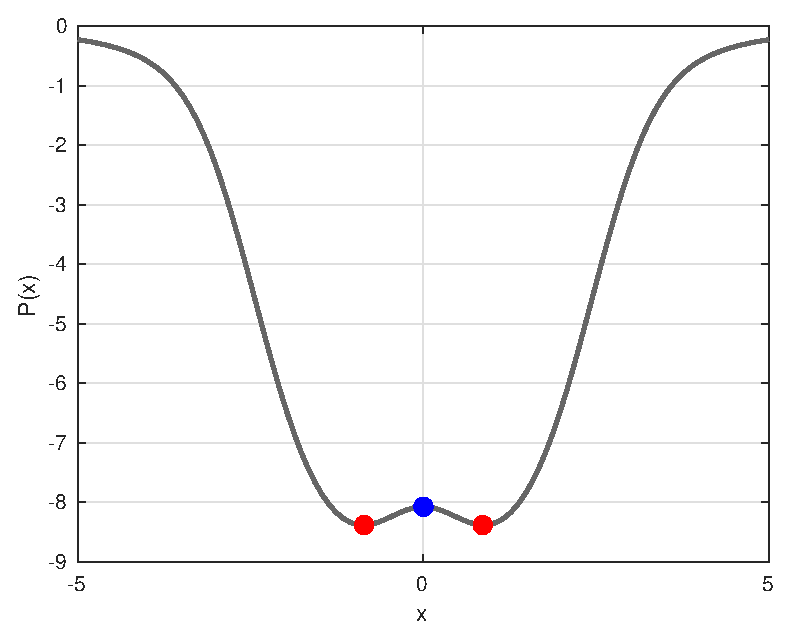
\includegraphics[scale=0.5]{img/Potential.eps} 
        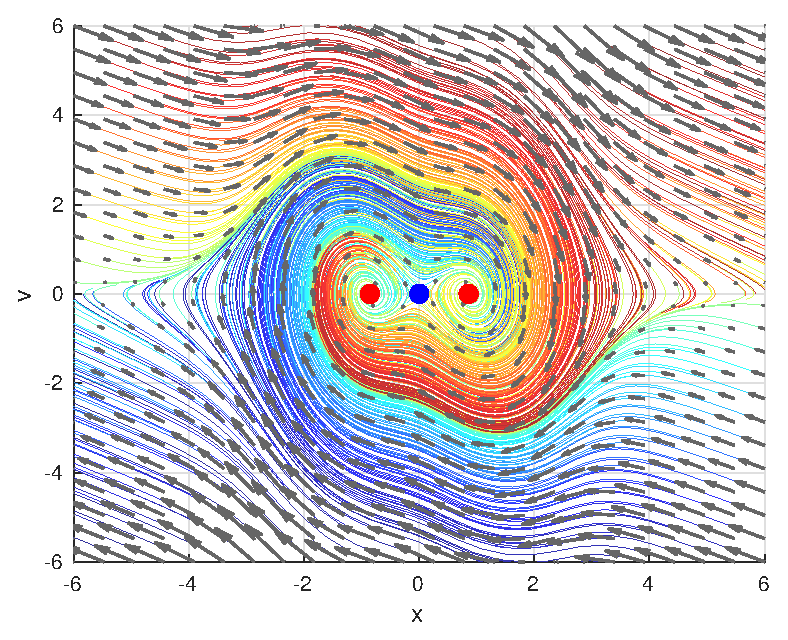
\includegraphics[scale=0.5]{img/pp_free.eps}
        \caption[Comportamiento de la partícula en un potencial]{
         A la izquierda se muestra el potencial en el que se mueve la partícula del ejemplo. Además a la derecha se muestra el comportamiento del espacio de fases del sistema. Alli estan dibujadas distintas trayectorias dentro del espacio de fases representadas con distintos colores. Podemos ver como todas las trayectorias acaban en los atractores representados por los puntos rojos, mientras que las trayectorias escapan del repulsor representado por el punto azul.}
        \label{fig:potencial}
    \end{figure}

    \begin{figure} 
        \centering
        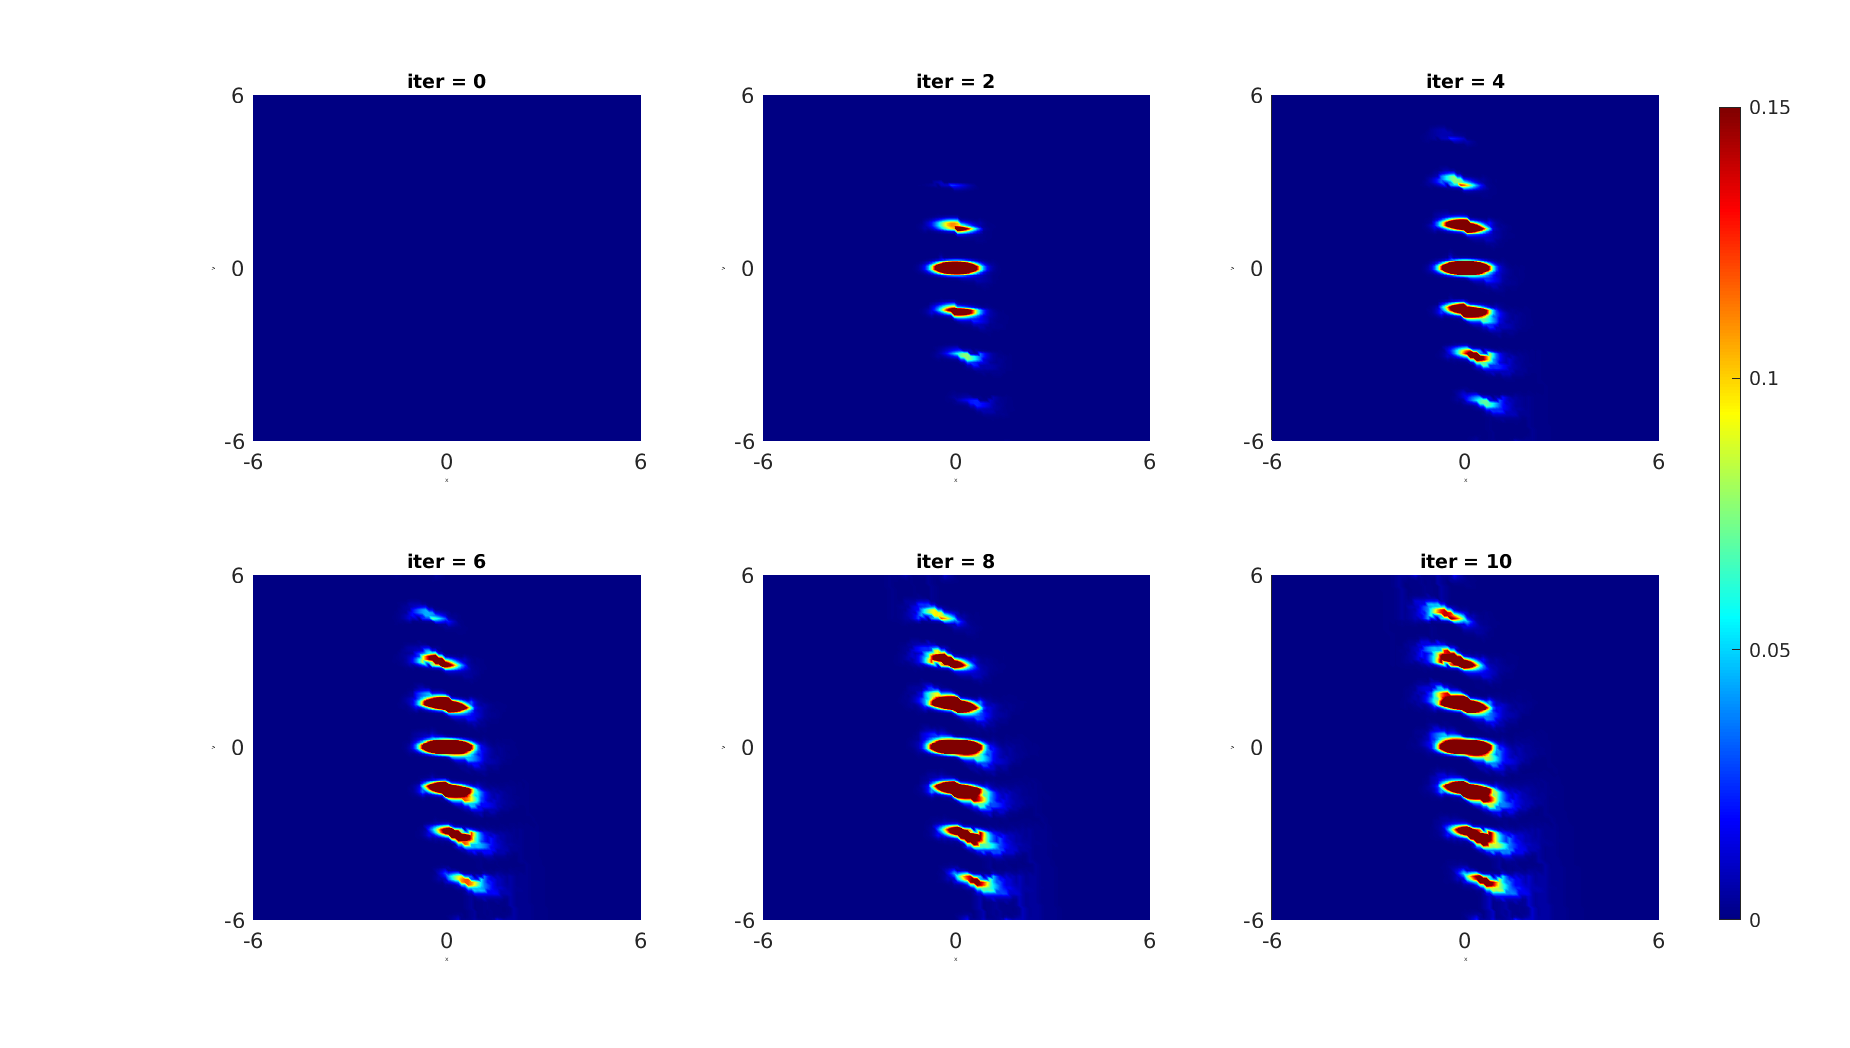
\includegraphics[scale=0.45]{img/valueiteration.eps}
        \caption[Evolución de la función vlaor por \emph{Value Iteration}]{Evolución de la función valor $\mathcal{V}_k(x,v)$ en distintas iteraciones del algoritmo  \emph{Q Iteration}. Podemos ver la convergencia de función valor de estado.}
        \label{fig:valueiteration}
    \end{figure} 

    \begin{figure} 
        \centering
        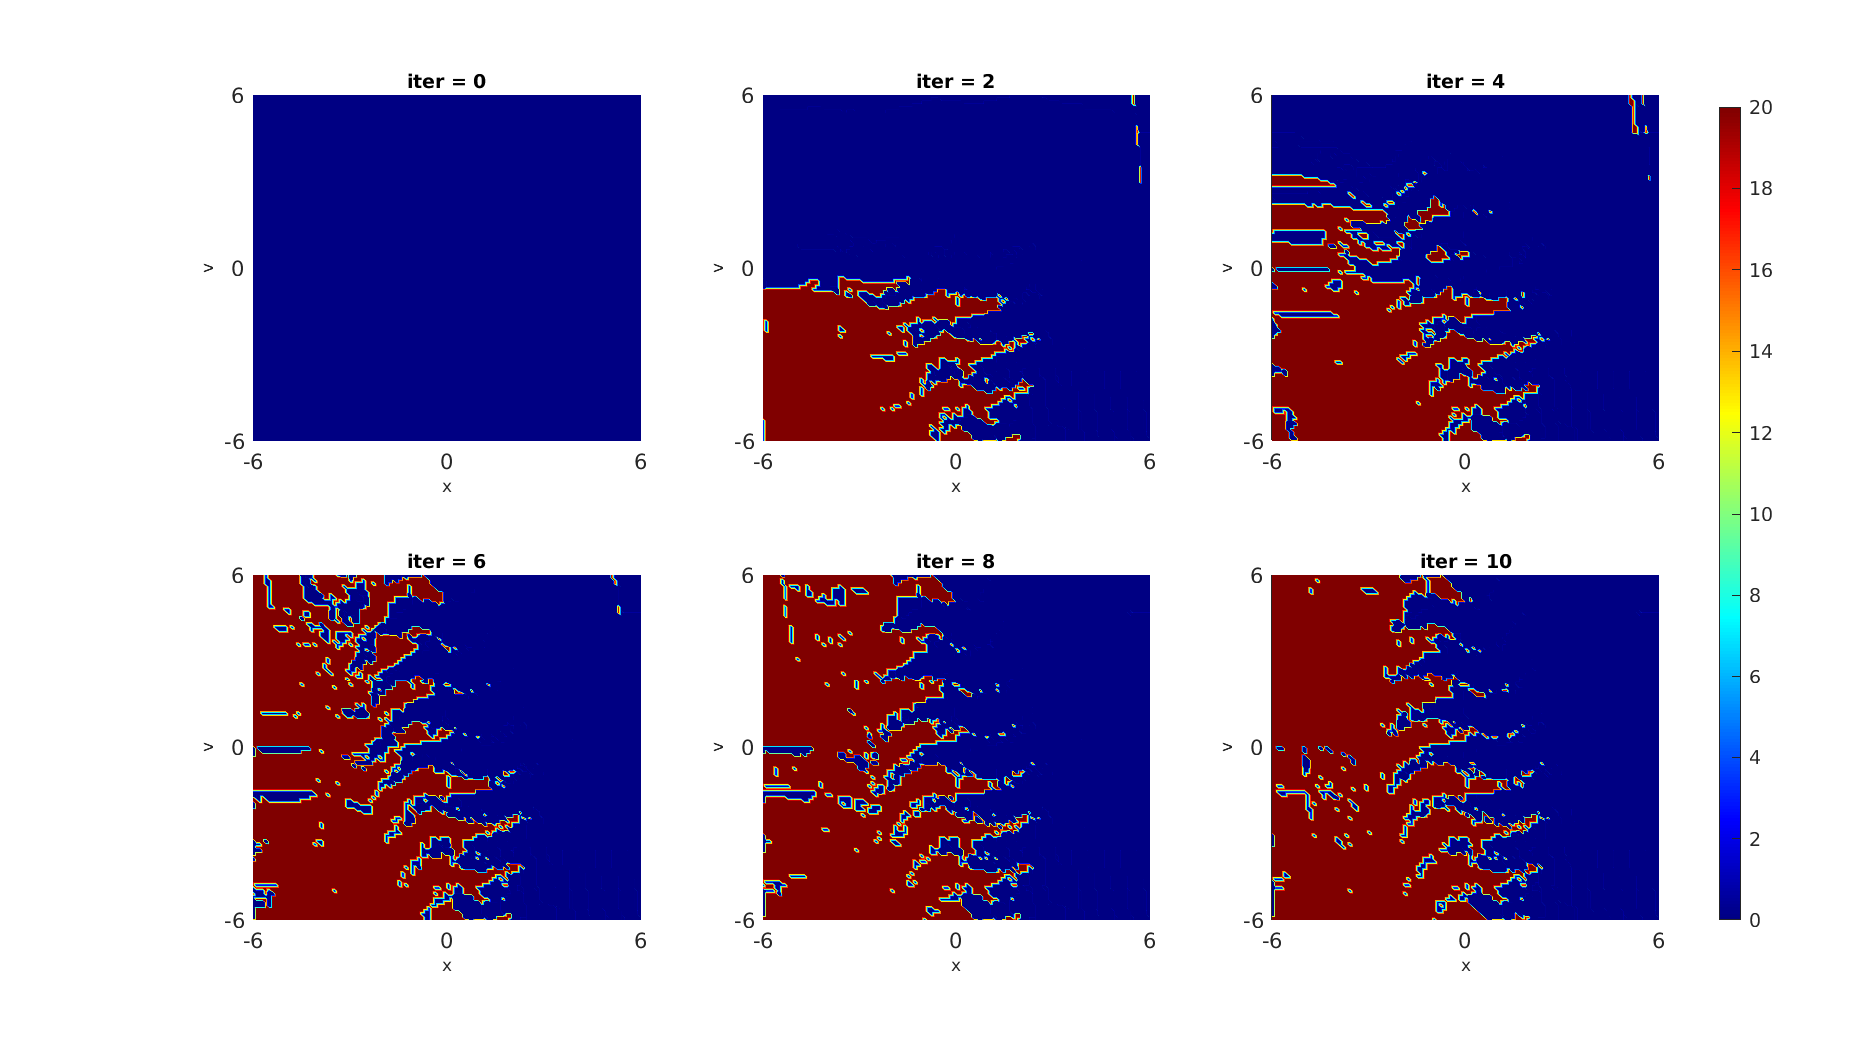
\includegraphics[scale=0.5]{img/valueiterationpi.eps}
        \caption[Evolución de la política por \emph{Value Iteration}]{
         Evolución de la política valor $\pi^*(x,v)$ en distintas iteraciones. Dado un punto del espacio de fases $(x,v)$ podemos obtener el valor de la acción. }
        \label{fig:piiteration}
    \end{figure} 

    \begin{figure}
        \centering
        \begin{subfigure}[b]{0.4\textwidth}
            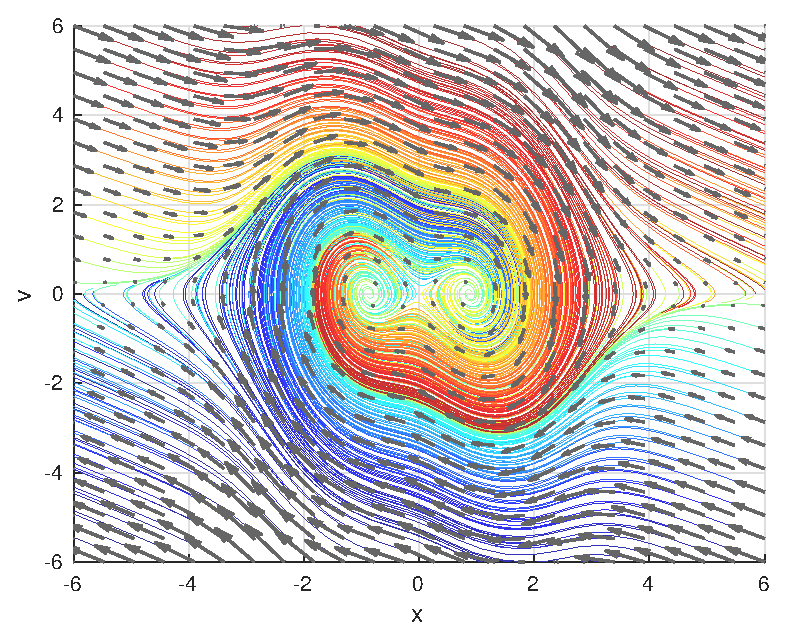
\includegraphics[width=\textwidth]{img/freepot.eps}
            \caption{Espacio de fases sin control}
            \label{afree}
        \end{subfigure}
        \begin{subfigure}[b]{0.4\textwidth}
            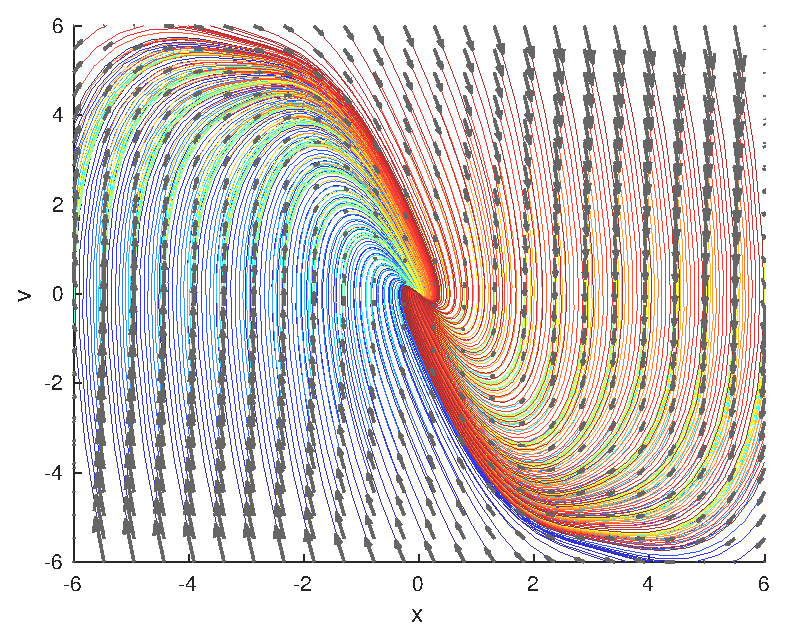
\includegraphics[width=\textwidth]{img/lqrpot.eps}
            \caption{Espacio de fases con LQR}
            \label{bLQR}
        \end{subfigure}
        \begin{subfigure}[b]{0.4\textwidth}
            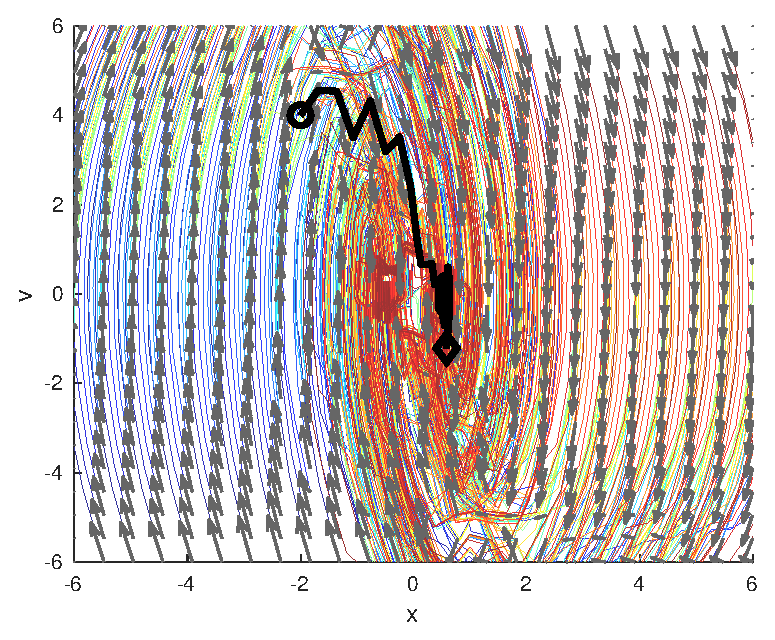
\includegraphics[width=\textwidth]{img/solpot.eps}
            \caption{Espacio de fases con \emph{Value Iteration}}
            \label{cQI}
        \end{subfigure}
        \begin{subfigure}[b]{0.4\textwidth}
            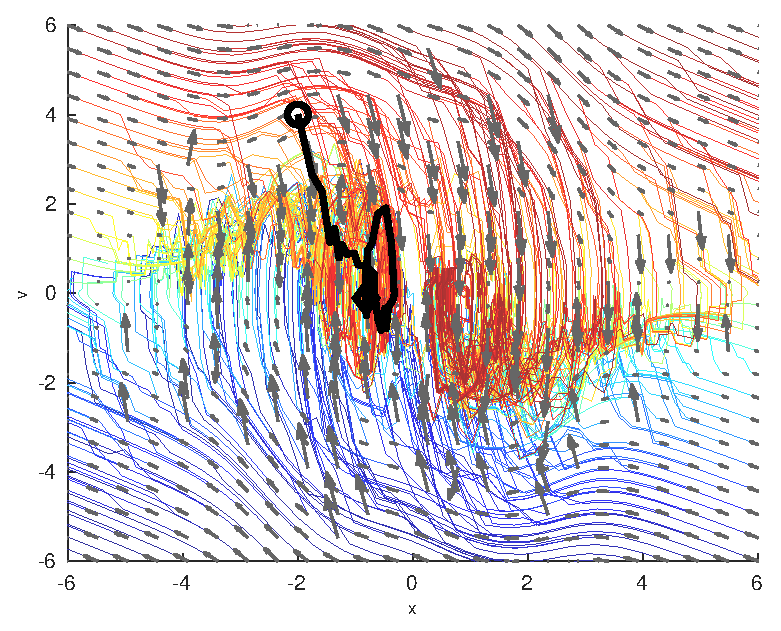
\includegraphics[width=\textwidth]{img/phase_Qlearning.eps}
            \caption{Espacio de fases con \emph{Q learning}}
            \label{cQI}
        \end{subfigure}
        
        \caption[Espacio de fases modificado]{
        Comparamos el espacio de fase del sistemas con la política obtenida mediante LQR (figura \ref{bLQR}), la política obtenida mediante el algoritmo \emph{Q-Iteration}  (figura \ref{cQI})y la dinámica libre (figura \ref{afree}).  }
        \label{fig:potencial}
    \end{figure}

\end{example}

%%%%%%%%%%%%%%%%%%%%%%%%%%%%%%%%%%%%%%%%%%%%%%%%%%%%%%%%%%%%%%%%%%%%%%%%%%%%%%%%%%%%%%%%%%%%%%%%%%%%%%%%%%%%%%%%%%%%%%%
%%%%%%%%%%%%%%%%%%%%%%%%%%%%%%%%%%%%%%%%%%%%%%%%%%%%%%%%%%%%%%%%%%%%%%%%%%%%%%%%%%%%%%%%%%%%%%%%%%%%%%%%%%%%%%%%%%%%%%%
%%%%%%%%%%%%%%%%%%%%%%%%%%%%%%%%%%%%%%%%%%%%%%%%%%%%%%%%%%%%%%%%%%%%%%%%%%%%%%%%%%%%%%%%%%%%%%%%%%%%%%%%%%%%%%%%%%%%%%%
